\section{Results}
%% i.e. validation against swiss norms
\subsection{Validation}
%%Chris
To validate the externality values estimated using MATSim, the produced outputs are analyzed both temporally and spatially to check for plausibility and then compared with the estimations from previous Swiss external cost reports.

\subsubsection{Emissions}
Emissions values can be estimated with MATSim directly from the processed GPS traces and therefore do not explicitely require a calibrated MATSim scenario for Switzerland.
Nevertheless, in order to validate our estimation, emission values are first calculated using a 10\% MATSim scenario for Switzerland.
To comply with new vehicle registrations statistics according to \cite{autoschweiz2010} and \cite{autoschweiz2012} as well as the vehicle ownership predictions from \cite{foen2010pollutants}, two scenarios where 30\% and 40\% of vehicles are assigned a diesel engine were examined.

The emission values are estimated for each road link in the MATSim network for the following pollutants: CO, total CO$_2$, FC, HC, NMHC, NO$_2$, NO$_x$, PM and SO$_2$.
The values are aggregated into hourly time bins.
These emission estimates are then first analyzed temporally and spatially to assure the plausibility of the output.

When analyzing the temporal evolution of emissions over the course of a typical workday, we would expect it to correlate with typical commuter patterns, i.e. low emissions both in the early morning and late evening and higher emissions during the day, with spikes corresponding to rush-hour periods.
\Cref{fig:hourlyEmissions} shows the typical daily emission of each pollutant per hourly time bin estimated from the MATSim scenario, for both the 30\% and 40\% diesel engine ownership scenarios.
Note that only total CO$_2$ and FC are shown, as the emissions values for the other pollutants are negligeable in comparison.
As expected, two distinct peaks corresponding to morning and evening rush-hours can be observed, while the early morning and late-night values are near zero and the midday values lie somewhere in between.

\createfigure%
{Hourly emissions values for Switzerland}%
{Hourly emissions values for Switzerland. Only total CO$_2$ and FC emissions are shown, as the values for the other pollutants are negligeable in comparison.}%
{\label{fig:hourlyEmissions}}%
{%
  \createsubfigure%
  {30\% diesel vehicles}%
  {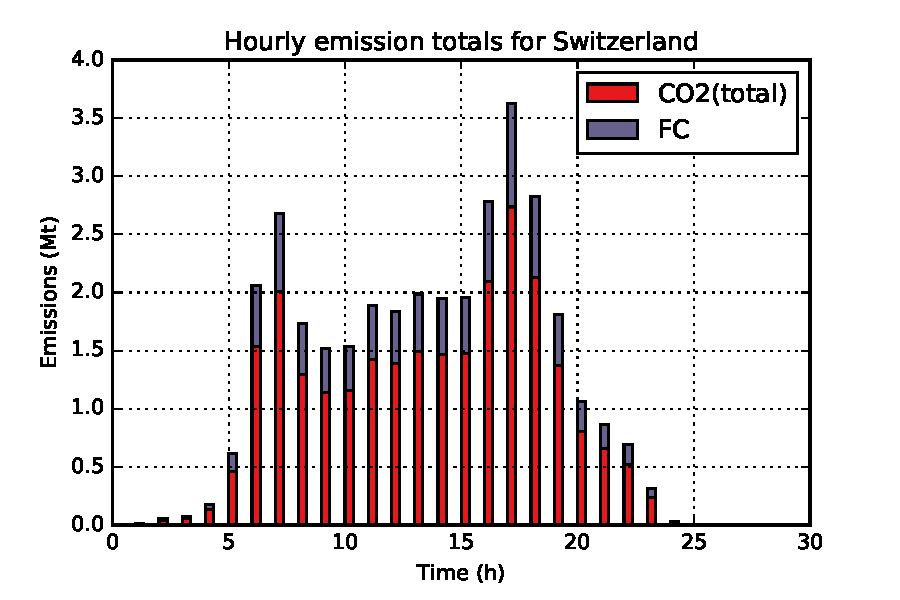
\includegraphics[width=0.49\textwidth,
angle=0]{figures/hourly_emissions_30pct_diesel.pdf}}%
  {\label{fig:hourlyEmissions-30pctDiesel}}%
  {}%
  \createsubfigure%
  {40\% diesel vehicles}%
  {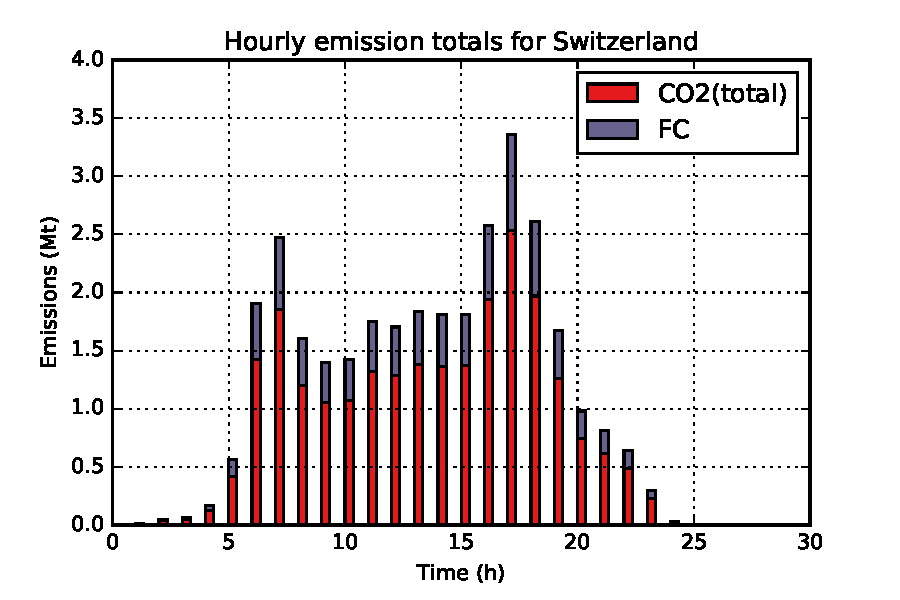
\includegraphics[width=0.49\textwidth,
angle=0]{figures/hourly_emissions_40pct_diesel.pdf}}%
  {\label{fig:hourlyEmissions-30pctDiesel}}%
  {}%
}%
{}

The spatial analysis of emissions is expected to show higher emissions in and around larger cities and within highly populated cantons, where more people live and therefore more commutes are observed.
Fig. shows the spatial distribution of the total daily emissions over entire Switzerland whereas Fig. show aggregated total daily emissions per canton.
Indeed, it can be seen that total emission values are higher in the main metropolitan areas (Zurich, Geneva, Basel, Bern, Lausanne, Lucerne, St-Gallen) than in rural areas within e.g. Graub\"unden, Valais, Schwyz or Appenzell.

\createfigure%
{Spatial distribution of total emissions in Switzerland}%
{Spatial distribution of total emissions in Switzerland}%
{\label{fig:spatialEmissions}}%
{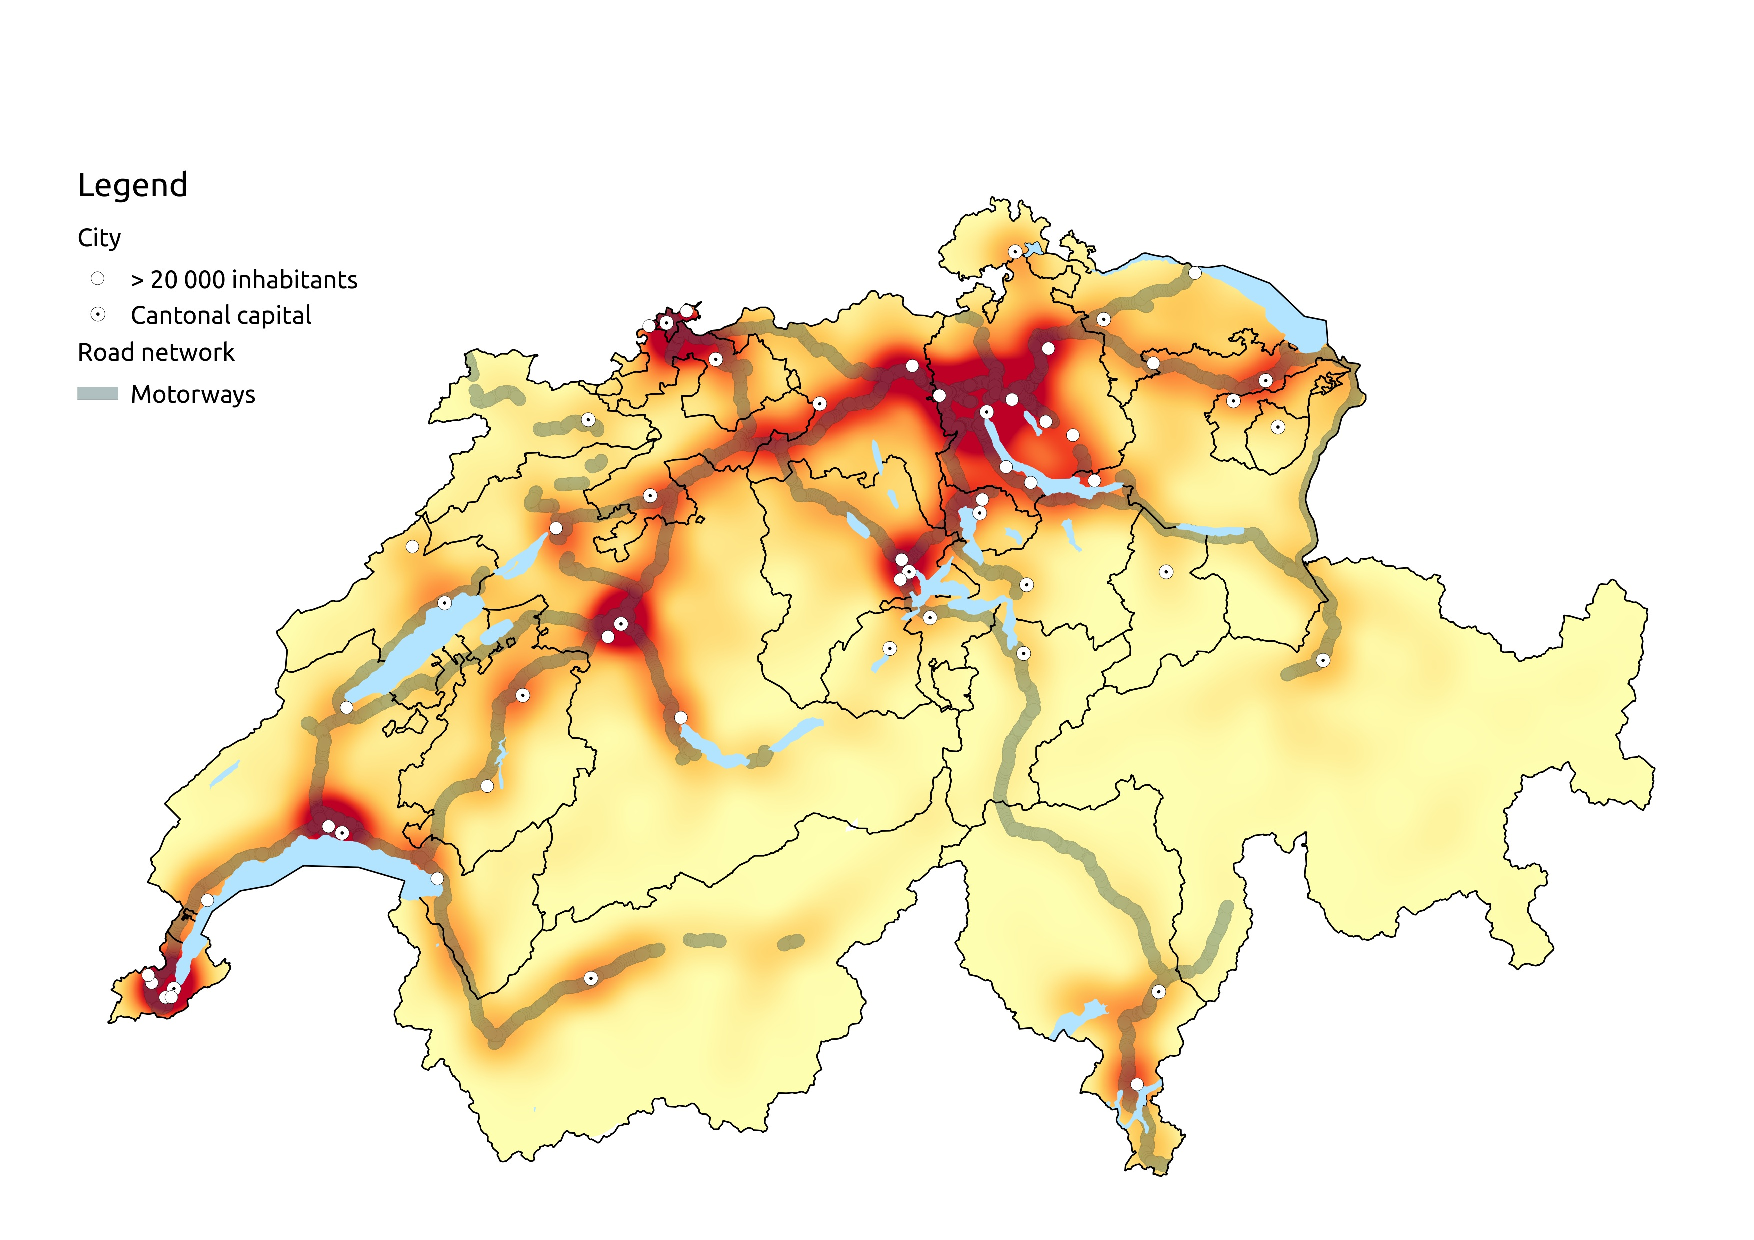
\includegraphics[width=1.0\textwidth, angle=0]{figures/total_emissions_heatmap.pdf}}%
{}

The MATSim computed emissions values are then compared to those calculated by \cite{foen2010pollutants} for 2015.
Since MATSim simulates a single typical workday for 10\% of the entire Swiss population, our values need to be scaled in order to be comparable.
The emissions values are thus multiplied by 10 to account for the population sampling, then by 365 days and finally by an additional scale factor such that the total traveled distance matches the one reported by \cite{foen2010pollutants} for 2015.
\Cref{tab:emissionValueMatsimFoenComparison} shows the total estimated emissions values for both MATSim scenarios and \cite{foen2010pollutants} and \Cref{fig:emissionValueMatsimFoenComparison} plots the percent deviation of the MATSim estimates from the reported 2015 estimates.
The total emission values for all pollutants except PM are within 20\% of the reported values with 30\% diesel engine ownership; they lie within 10\% in the 40\% diesel engine ownership case.
These deviations are possibly due to the fact that emissions factors depend on the exact type of petrol or diesel engine.
In the MATSim model, only one type of petrol and diesel engine is considered, whereas in reality, these are further subdivided into specific subtypes.
Further calibration of the vehicle engine types to the appropriate subtypes could possibly lead to a better fit in emissions values.
Nevertheless, the estimed values are coincide with the previously reported values, thereby demonstrating that MATSim provides a reliable means of estimating emission values for pollutants.

TODO:
mention something of the review of engine fleet and effect on PM?
maybe compare also to 2004 report?

\createtable%
{MATSim and FOEN estimated emission value comparison}%
{MATSim and FOEN estimated emission value comparison}%
{\label{tab:emissionValueMatsimFoenComparison}}%
{%
  \begin{tabular}[c]{lrrrrr}
    \toprule
    \multirow{3}{*}{Pollutant} & \multirow{3}{*}{FOEN} & \multicolumn{4}{c}{MATSim} \\ 
    & & \multicolumn{2}{c}{30\% diesel} & \multicolumn{2}{c}{40\% diesel}\\
    & t/a & t/a & \% & t/a & \% \\
    \midrule
    CO$_2$(total) & 10 687 911 & 11 770 667 &  10.13 &  10 893 138 &   1.92 \\
    FC &                    NA &  3 872 146 &    --- &   3 582 233 &    --- \\
    CO &                67 424 &     69 526 &   3.12 &      61 283 &  -9.11 \\
    NOx &               16 496 &     14 004 & -15.11 &      17 220 &   4.39 \\
    HC &                 9 546 &      9 820 &   2.87 &       8 777 &  -8.06 \\
    NMHC &               9 037 &      9 291 &   2.81 &       8 315 &  -7.98 \\
    NO2 &                4 127 &      3 410 & -17.38 &       4 471 &   8.34 \\
    PM &                   418 &        523 &  25.16 &         672 &  60.85 \\
    SO2 &                   59 &         57 &  -3.56 &          53 & -10.48 \\
    \bottomrule
  \end{tabular}
}%
{}

\createfigure%
{MATSim and FOEN estimated emission value comparison}%
{MATSim and FOEN estimated emission value comparison}%
{\label{fig:emissionValueMatsimFoenComparison}}%
{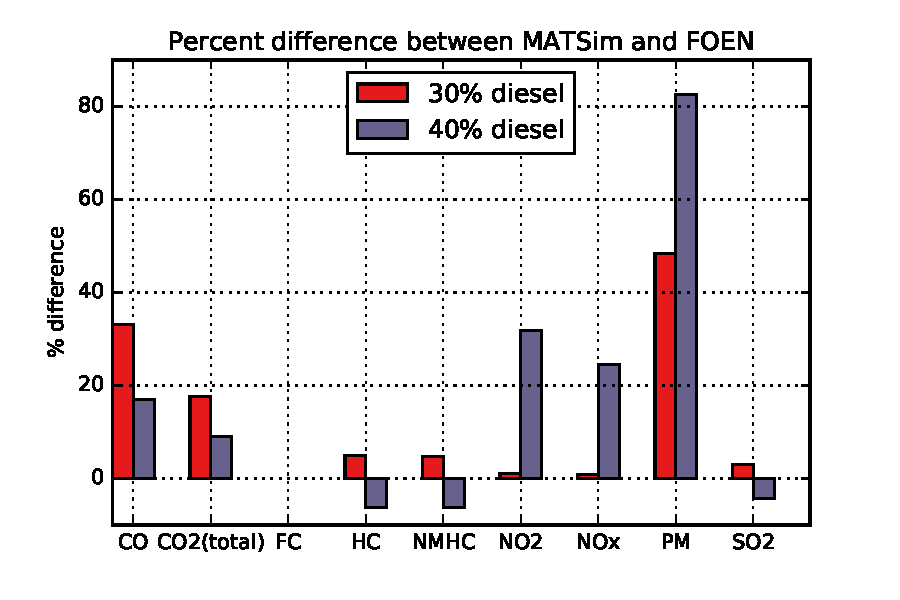
\includegraphics[width=1.0\textwidth, angle=0]{figures/percent_differences.pdf}}%
{}

\subsubsection{Congestion}

Contrary to emissions, congestion and delays caused to others cannot directly be estimated from GPS traces alone, since information on how many other drivers were present on the road at that given moment is lacking.
It is precisely for this reason that MATSim is used to estimate congestion throughout a typical workday.
Therefore, it is crucial that the estimated aggregate congestion values are consistent with other previous estimates.
As before, these values are calculated using a 10\% MATSim scenario for Switzerland and are aggregated into hourly time bins per road link.
These estimates are again first analyzed temporally and spatially to assure the plausibility of the output before being compared to \cite{mkinfras2016staukosten}.

The typical total caused delays pattern per hourly time bin estimated from the MATSim scenario is shown in \Cref{fig:hourlyDelays}.
As was the case for emissions, total delays also expectedly coincide with typical commuter patterns, with fewer delays the early morning and at night, two distinct peaks corresponding to morning and evening rush-hours and midrange values at midday.

\createfigure%
{Hourly total caused delays for Switzerland}%
{Hourly total caused delays for Switzerland}%
{\label{fig:hourlyDelays}}%
{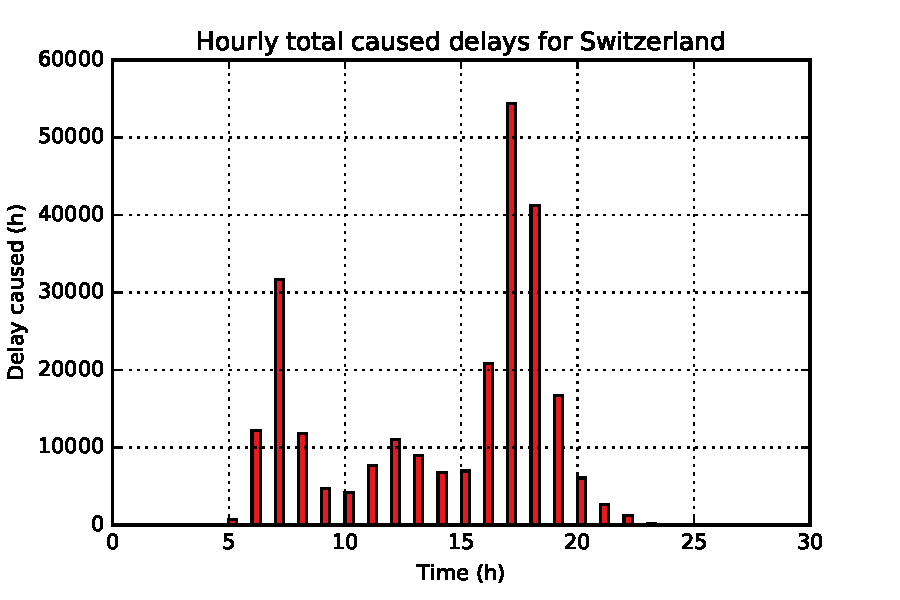
\includegraphics[width=0.8\textwidth,
angle=0]{figures/hourly_caused_delays.pdf}}%
{}

\Cref{fig:hourlyDelays} shows the spatial distribution of the total daily caused delays over entire Switzerland.
Following an anogolous reasoning as for emissions, longer delay times are observed in and around larger cities and within highly populated cantons, where more people live and commute to.

\createfigure%
{Spatial distribution of total emissions in Switzerland}%
{Spatial distribution of total emissions in Switzerland}%
{\label{fig:spatialDelays}}%
{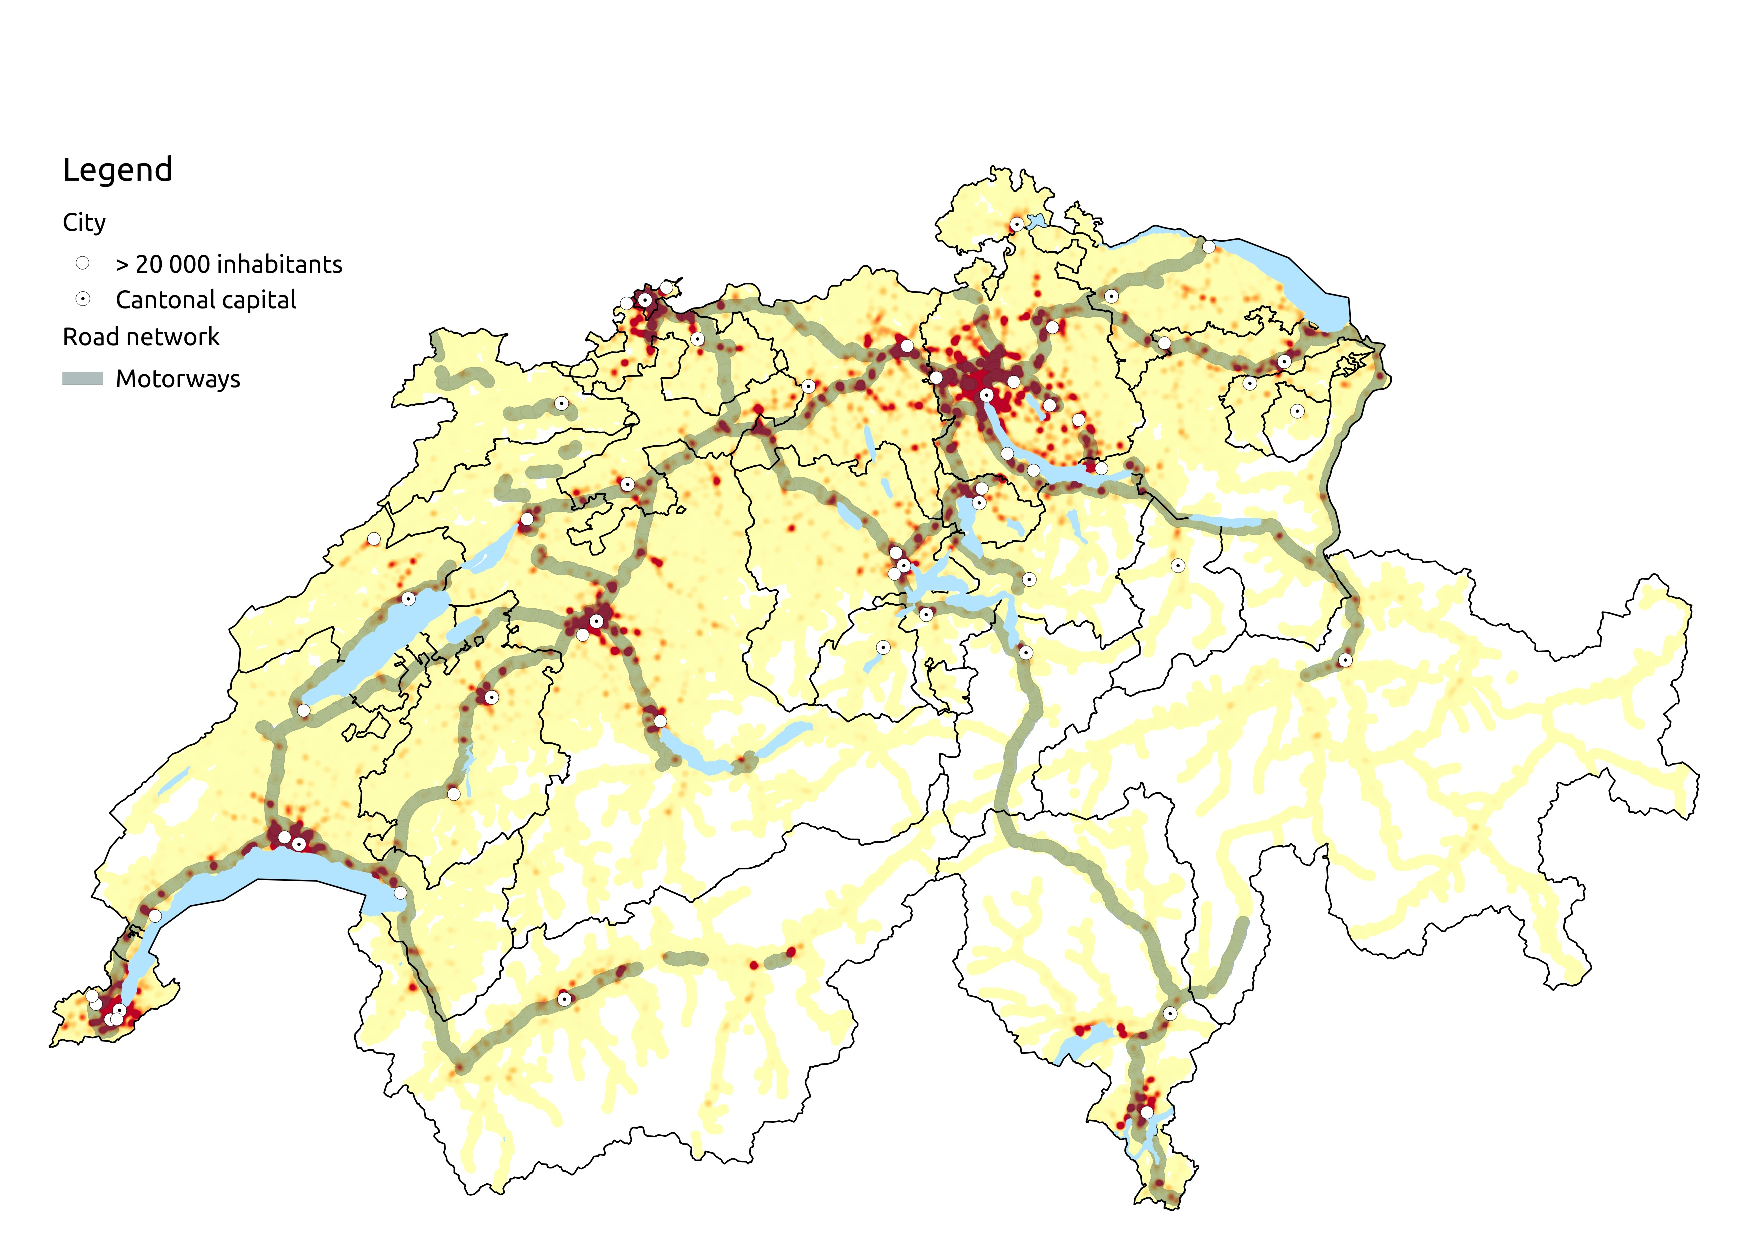
\includegraphics[width=1.0\textwidth, angle=0]{figures/total_delays_heatmap.pdf}}%
{}

The MATSim computed delay values are then compared to those calculated by \cite{mkinfras2016staukosten}.
The same scaling operations are performed as in the case of emissions: multiplication by 10 to account for the population sampling, then by 365 days and finally by an additional scale factor such that the total traveled distance matches the one reported by \cite{foen2010pollutants} for 2015.
The values are reported in \Cref{tab:delayValueComparison}.


\createtable%
{MATSim and Infras / MK Consulting congestion comparison}%
{MATSim and Infras / MK Consulting congestion comparison}%
{\label{tab:delayValueComparison}}%
{%
  \begin{tabular}[c]{lrrr}
    \toprule
    Road type & MK/Infras (Mveh-h/a) & MATSim (Mveh-h/a) & \%  \\ 
    \midrule
    Motorway      & 16.62 &    8.33 &  -49.8901 \\
    Non-motorway  & 11.23 &   95.00 &  745.9803 \\
    Total &         27.85 &  103.33 &  271.0300 \\
    \bottomrule
  \end{tabular}
}%
{}

The total vehicle hour delay per year values are estimated to be much higher in MATSim than in the report.
However, the authors do indeed state that they have taken an "at-least" approach in estimating delays and that the values for non-motorway segments are highly underestimated.
On the other hand, our model only similulates passengers vehicles.
Therefore, it neither accounts for the effects of the interaction of cars with trucks on motorways nor does it captures extraordinary circumstances such as accidents and holiday traffic which could increase the vehicle hours of delay.
A combination of these effects could be the underlying cause of the deviation between the estimates and should be further examined.


\subsection{Green Class Emission Reductions}
A core component of the Green Class pilot project was the availability of an electric car to subscribers. 
As trip data records whether a personal vehicle or the electic vehicle was used, the emission reductions resulting from the provision of the electric vehicles can be measured. Two key assumptions must however be made and noted:
\begin{enumerate}
  \item The driving behaviour is independent of the drive-train type.
  \item Participants only switched their chosen type of vehicle, and would have made the trip anyway, at the same time, even without the Green Class subscription.
  \end{enumerate}

In figure \cite{fig:green-class-reduction} the reduction in emissions of the course of the program due to the availability of the E-car is illustrated. 
A clear immediate reduction in CO\textsubscript{2} is observed. Overall, from the pre-Ecar period, a reduction of 30\% can be observed. 
There are some noticable outliers, particularly April 1\textsuperscript{st}, 2017. 
In the pilot program, subscribers had unrestricted access to both thier personal vehicle and the provided electric vehicle. 
As such, on days where many subscribers choose to use thier personal vehicles, emissions will naturally be nearer to the pre-program levels. 
A particular reason for this would be public holidays where many subscribers are likely to want to travel further than allowed with the range of the electric vehicle.

\createfigure%
{Percentage of pre electric vehicle CO \textsubscript{2} produced per day. EV's were provided on January 16, 2017. }%
{Percentage of pre electric vehicle CO \textsubscript{2} produced per day. EV's were provided on January 16, 2017. }%
{\label{fig:green-class-reduction}}%
{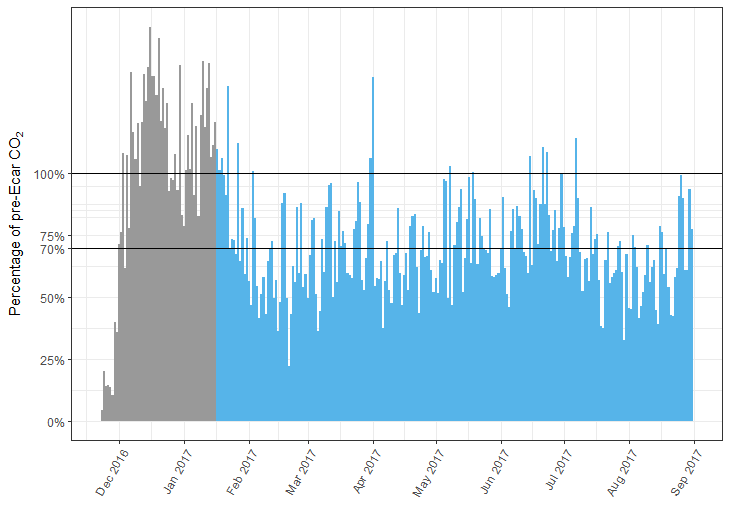
\includegraphics[width=1.0\textwidth, angle=0]{figures/green_class_pollutant_reductions_daily}}%
{}

%%%%%%TODO: add a comparison of congestion experienced vs congsetion caused for green class drivers